\documentclass[12pt, a4paper]{report}
\usepackage[utf8]{inputenc}
\usepackage[english, russian]{babel}

\usepackage{graphicx}
\usepackage{listings}
\usepackage{color}

\usepackage{amsmath}
\usepackage{pgfplots}
\usepackage{url}
\usepackage{flowchart}
\usepackage{tikz}
\DeclareGraphicsExtensions{.pdf,.png,.jpg,.svg}
\usetikzlibrary{shapes, arrows}

\usepackage{pgfplotstable}

\renewcommand\contentsname{Содержание}

\usepackage{geometry}
\geometry{left=3cm}
\geometry{right=1cm}
\geometry{top=2cm}
\geometry{bottom=2cm}

\lstset{ %
language=C++,                 % выбор языка для подсветки (здесь это С)
basicstyle=\small\sffamily, % размер и начертание шрифта для подсветки кода
numbers=left,               % где поставить нумерацию строк (слева\справа)
numberstyle=\tiny,           % размер шрифта для номеров строк
stepnumber=1,                   % размер шага между двумя номерами строк
numbersep=-5pt,                % как далеко отстоят номера строк от         подсвечиваемого кода
backgroundcolor=\color{white}, % цвет фона подсветки - используем         \usepackage{color}
showspaces=false,            % показывать или нет пробелы специальными     отступами
showstringspaces=false,      % показывать или нет пробелы в строках
showtabs=false,             % показывать или нет табуляцию в строках
frame=single,              % рисовать рамку вокруг кода
tabsize=2,                 % размер табуляции по умолчанию равен 2 пробелам
captionpos=t,              % позиция заголовка вверху [t] или внизу [b] 
breaklines=true,           % автоматически переносить строки (да\нет)
breakatwhitespace=false, % переносить строки только если есть пробел
escapeinside={\%*}{*)},   % если нужно добавить комментарии в коде
keywordstyle=\color{blue}\ttfamily,
stringstyle=\color{red}\ttfamily,
commentstyle=\color{green}\ttfamily,
morecomment=[l][\color{magenta}]{\#},
columns=fullflexible }

\usepackage{titlesec}
\titleformat{\chapter}[hang]{\LARGE\bfseries}{\thechapter{.} }{0pt}{\LARGE\bfseries}
\titleformat*{\section}{\Large\bfseries}
\titleformat*{\subsection}{\large\bfseries}

\begin{document}

    \begin{titlepage}

        \begin{center}
            \Large
            {\sl Государственное образовательное учреждение высшего профессионального образования\\
            {\bf«Московский государственный технический университет имени Н.Э. Баумана»\\
				(МГТУ им. Н.Э. Баумана)}}
				\noindent\rule{\textwidth}{2pt}
            \vspace{3cm}

			{\scshape\LARGE Лабораторная работа №2 \par}
			\vspace{0.5cm}	
			{\scshape\LARGE по курсу «Анализ алгоритмов» \par}
			\vspace{1.5cm}
			{\huge\bfseries Сортировка массивов \par}
			\vspace{2cm}
			\Large Выполнил: Сорокин А.П., гр. ИУ7-52Б\\
			\vspace{0.5cm}
			{\Large Преподаватели: Волкова Л.Л., Строганов Ю.В.}
		
			\vfill
			\Large \textit {Москва, 2019 г.}
            
        \end{center}

    \end{titlepage}
	
	\tableofcontents

	\chapter*{Введение}
	\addcontentsline{toc}{chapter}{Введение}
	
	В настоящее время в любом программном проекте необходимо обрабатывать большое число однотипных данных. Такие данные удобно обрабатывать, используя массив - именнованную последовательность однотипных данных. Благодаря тому, что элементы массива расположены последовательно, упрощается их обработка.
	Очень часто требуется сортировать данные по какому-либо признаку, или ключу. В отсортированных массивах значительно быстрее можно выполнять поиск определённых данных по ключу. Существует множество алгоритмов сортировки массивов, которые применяются при различных условиях в зависимости от задач, стоящих перед программой. В данной лабораторной работе изучаются некоторые из алгоритмов сортировки массивов на предмет их эффективности.
	
    \chapter{Аналитическая часть}
	\section{Задачи}
	Цель лабораторной работы - изучение трех алгоритмов сортировки массивов. Были выбраны следующие алгоритмы:
	\begin{itemize}
		\item сортировка вставками;
		\item сортировка слиянием;
		\item быстрая сортировка.
	\end{itemize}
	Для того чтобы добиться поставленной цели, были поставлены следующие задачи:
	\begin{itemize}
		\item изучить и реализовать алгоритмы сортировок массивов;
		\item оценить трудоёмкости алгоритмов;
		\item выполнить сравнительный анализ алгоритмов на основе трудоёмкости и используемой памяти;
		\item оценить и сравнить эффективности алгоритмов по времени.
	\end{itemize}

	\section{Описание алгоритмов}
	На вход алгоритмов подаётся последовательность n чисел $a_1, a_2, a_3,.., a_N$. Сортируемые числа также называют ключами. Входная последовательность на практике представляется в виде массива с $N$	элементами. На выходе алгоритмы должны вернуть перестановку исходной последовательности $a'_1, a'_2, a'_3,.., a'_N$, чтобы выполнялось соотношение $a'_1 \leq a'_2 \leq ...\leq a'_N$\\
	
	\subsection{Сортировка вставками}
	В алгоритме сортировки вставками элементы входной последовательности просматриваются по одному, и каждый новый поступивший элемент размещается в подходящее место среди ранее упорядоченных элементов.\\
	В начальный момент отсортированная последовательность пуста. На каждом шаге алгоритма выбирается один из элементов входных данных и помещается на нужную позицию в уже отсортированной последовательности до тех пор, пока набор входных данных не будет исчерпан. В любой момент времени в отсортированной последовательности элементы удовлетворяют требованиям к выходным данным алгоритма.

	\subsection{Сортировка слиянием}
	В алгоритме сортировки слиянием массив разбивается на два массива одинакового размера (от среднего элемента). Каждая из этой частей разбивается таким же образом до тех пор, пока длина массива не станет равной 1. Затем выполняется слияние двух подмассивов: на каждом шаге берётся меньший из двух первых элементов подмассивов и записывается в результирующий. Счётчики номеров элементов результирующего массива и подмассива, из которого был взят элемент, увеличиваем на 1. Как только заканчивается один из подмассивов, оставшиеся элементы второго записываются в конец результирующего. ~\cite{Merge}
		
	\subsection{Быстрая сортировка}
	В алгоритме быстрое сортировки исходный массив разбивается на два отрезка по опорному элементу: на одном отрезке находятся все элементы, меньшие опорного, во втором - большие (или равные). Для выставления правильного порядка относительно опорного элемента выполняется перестановка. При этом в массиве в начале идёт отрезок, в котором расположены меньшие элементы, а затем - в котором большие или равные. Затем для каждого из этих отрезков выполняется то же разбиение рекурсивно. Разделение на отрезка продолжается, пока длина отрезка больше единицы. ~\cite{Quick}
	
	\subsection{Модель вычислений}
	В рамках данной работы используется следующая модель вычислений:
	\begin{itemize}
		\item операции, имеющие трудоемкость 1: $<$, $>$, $=$, $<=$, $=>$, $==$, $!=$,$+$, $-$, $\ast$, /, $+$=, $-$=, $\ast$=, $/$=, [ ];
		\item оператор условного перехода имеет трудоёмкость, равную трудоёмкости операторов тела условия;
		\item оператор цикла for имеет трудоемкость:
		\begin{equation}
		\label{for_cost}
		F_{for} = F_{init} + F_{check} + N \ast (F_{body} + F_{inc} + F_{check}),
		\end{equation}
		где $F_{init}$ -- трудоёмкость инициализации, $F_{check}$ -- трудоёмкость проверки условия, $F_{inc}$ -- трудоёмкость инкремента аргумента, $F_{body}$ -- трудоёмкость операций в теле цикла, $N$ -- число повторений. ~\cite{AlgAnalysis}
	\end{itemize} 
	

	\chapter{Конструкторская часть}
	
	\section{Схемы алгоритмов}
	На рисунках \ref{pic:insert}, \ref{pic:merge}, \ref{pic:quick} представлены схемы алгоритмов трёх алгоритмов сортировки массивов. Сортировка выполняется по возрастанию.
	\begin{figure}[ht!]
		\centering
		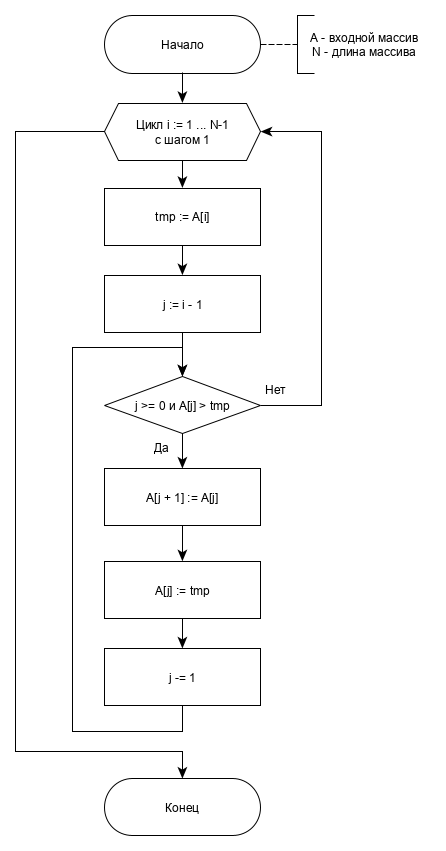
\includegraphics[scale=0.55]{insert.png}
		\caption{Схема алгоритма сортировки вставками}
		\label{pic:insert}
	\end{figure}
	\newpage
	\begin{figure}[ht!]
		\centering
		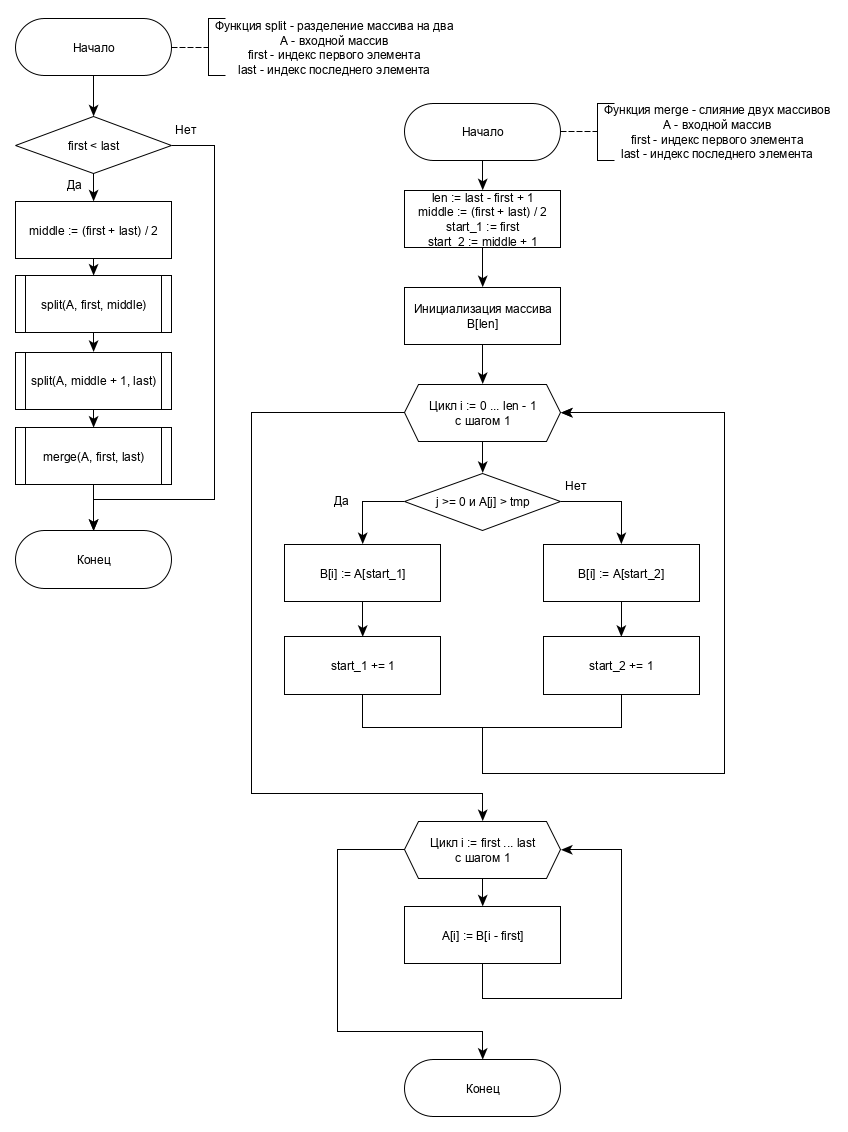
\includegraphics[scale=0.55]{merge.png}
		\caption{Схема алгоритма сортировки слиянием}
		\label{pic:merge}
	\end{figure}
	\newpage
	\begin{figure}[ht!]
		\centering
		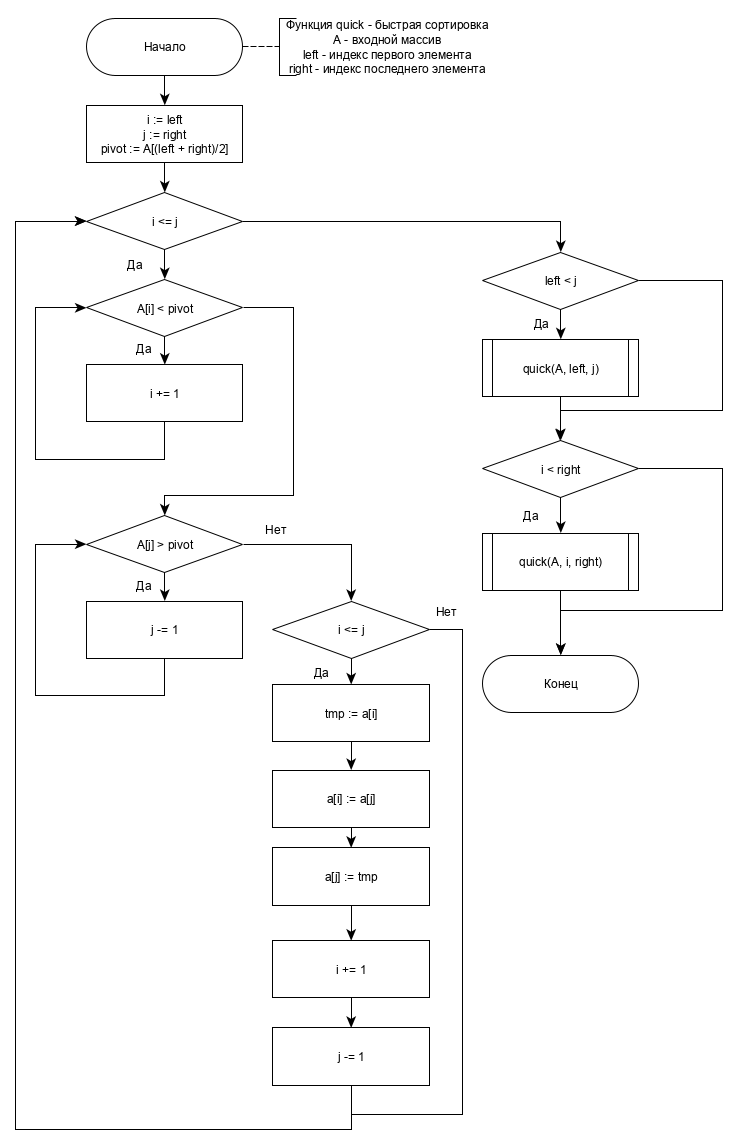
\includegraphics[scale=0.55]{quick.png}
		\caption{Схема алгоритма быстрой сортировки}
		\label{pic:quick}
	\end{figure}

	\newpage

	\section{Оценка трудоёмкости}
	Пусть дан массив $A$ длиной $N$. Рассмотрим трудоемкость трёх алгоритмов сортировки.
	
	\subsection{Сортировка вставками}
	\begin{enumerate}
		\item Худший случай - массив отсортирован в обратном порядке:
		\begin{itemize}
			\item Число сравнений в теле цикла: $(N-1)\frac{N}{2}$
			\item Число сравнений в заголовках циклов: $(N-1)\frac{N}{2}$
			\item Общее число сравнений: $(N-1)N$
			\item Число присваиваний в заголовках циклов: $(N-1)\frac{N}{2}$
			\item Число обменов: $(N-1)\frac{N}{2}$\\
			\item Итоговая трудоёмкость: $2(N-1)N = 2N^2 - N$
		\end{itemize}
		\item Лучший случай - массив уже отсортирован:
		\begin{itemize}
			\item Число сравнений в теле цикла: $(N-1)\frac{N}{2}$
			\item Число сравнений в заголовках циклов: $(N-1)\frac{N}{2}$
			\item Общее число сравнений: $(N-1)N$
			\item Число присваиваний в заголовках циклов: $(N-1)\frac{N}{2}$
			\item Число обменов: $0$\\
			\item Итоговая трудоёмкость: $\frac{3}{2}(N-1)N = \frac{3}{2}N^2 - \frac{3}{2}N$
		\end{itemize}
	\end{enumerate}
	
	\subsection{Сортировка слиянием}
	И в худшем, и в лучшем случаях число операций глубина рекурсии $h = logN$:
	\begin{itemize}
		\item Трудоёмкость разбиения: $5$
		\item Трудоёмкость инициализации пределов и середины: $9$
		\item Трудоёмкость цикла слияния: $2 + N\cdot(15 + 2) = 2 + 17N$
		\item Трудоёмкость переноса результат слияния: $2 + N\cdot(3 + 2) = 5N + 2$\
		\item Итоговая трудоёмкость: $logN\cdot(5 + 9 + 2 + 17N + 5N + 2) = 22NlogN + 18logN$
	\end{itemize}
	
	\subsection{Быстрая сортировка}
		\begin{enumerate}
		\item Худший случай - каждый раз выбирается один отрезок длиной 1:
		\begin{itemize}
			\item Глубина рекурсии: $h = N$
			\item Выбор опорного элемента: $4$
			\item Трудоёмкость цикла: $2 + N\cdot(2 + 1)=3N + 2$
			\item Перестановка элементов: $10$\\
			\item Итоговая трудоёмкость: $N\cdot(3N + 16) = 3N^2 + 16N$
		\end{itemize}
		\item Лучший случай - каждый раз массив разделяется на два одинаковых по длине отрезка:
		\begin{itemize}
			\item Глубина рекурсии: $h = logN$
			\item Выбор опорного элемента: $4$
			\item Трудоёмкость цикла: $2 + 2\cdot\frac{N}{2}\cdot(2 + 1)=3N + 2$
			\item Перестановка элементов: $10$\\
			\item Итоговая трудоёмкость: $logN\cdot(3N + 16) = 3NlogN + 16logN$
		\end{itemize}
	\end{enumerate}

	\section{Замер используемой памяти}
	В каждом из алгоритмов требуется хранить исходный массив $A$ длиной $N$. Таким образом, под хранение массива требуется $N$ байт памяти.\\
	Однако рекурсивные алгоритмы сортировки при любых случаях требуют использование дополнительной памяти под временное хранение элементов массива. Длина таких временных массивов зависит от N.
	
	\section{Сравнительный анализ алгоритмов}
	Исходя из проведённых анализов, можно заметить, что несмотря на то, что алгоритм вставками не использует большое количество дополнительной памяти (только под итераторы циклов), данный алгоритм уступает в трудоёмкости в лучших случаях рекурсивным алгоритмам сортировки слиянием и быстрой сортировки. Однако данные рекурсивные алгоритмы требуют дополнительно память, соизмеримую с размером массива (напрямую зависит от N).\\
	Также стоит отметить, что выбор опорного элемента в алгоритме быстрой сортировки может коренным образом повлиять на трудоёмкость алгоритма. В худшем случае данный алгоритм уступает алгоритму вставками и по трудоёмкости, и по памяти.
	
	
	\chapter{Технологическая часть}
	\section{Требования к программному обеспечению}
	На вход подаются размер массива и сам массив. На выход программа выдаёт три массива, которые являются результатами работы трёх различных алгоритмов сортировки. Сортировка выполняется по возрастанию.
	\section{Средства реализации}
	Для реализации программы был использован язык C++ ~\cite{CPP}. Для замера процессорного времени была использована функция rdtsc() из библиотеки stdrin.h.
	\section{Реализации алгоритмов}
	В листингах \ref{code-insert}, \ref{code-merge}, \ref{code-quick} представлены коды реализации алгоритмов сортировки массивов.
	\begin{lstlisting}[label=code-insert,caption=Сортировка вставками]
	void array_sort_insert(int * const arr, size_t n)
	{
		for (size_t i = 1; i < n; i++)
		{
			int tmp = arr[i];
			int j = i - 1;
			while (j >= 0 && arr[j] > tmp)
			{
				arr[j + 1] = arr[j];
				arr[j] = tmp;
				j--;
			}
		}
	}
	\end{lstlisting}

	\begin{lstlisting}[label=code-merge,caption=Сортировка слиянием]
	void array_merge(int * const arr, size_t first, size_t last)
	{
		size_t len = last - first + 1;
		size_t middle = (first + last) / 2;
		size_t start_1 = first;
		size_t start_2 = middle + 1;
		
		int *arr_tmp = new int[len];
		
		for (size_t i = 0; i < len; i++)
			if ((start_1 <= middle) && ((start_2 > last) ||
				(arr[start_1] < arr[start_2])))
			{
				arr_tmp[i] = arr[start_1];
				start_1++;
			}
			else
			{
				arr_tmp[i] = arr[start_2];
				start_2++;
			}
		
		for (size_t i = first; i <= last; i++)
			arr[i] = arr_tmp[i - first];
		delete [] arr_tmp;
	}
	
	void array_sort_merge(int * const arr, size_t first, size_t last)
	{
		if (first < last)
		{
			size_t middle = (first + last) / 2;
			array_sort_merge(arr, first, middle);
			array_sort_merge(arr, middle + 1, last);
			array_merge(arr, first, last);
		}
	}
	\end{lstlisting}

	\begin{lstlisting}[label=code-quick,caption=Быстрая сортировка]
	void array_sort_quick(int * const arr, size_t left, size_t right)
	{
		unsigned i = left, j = right;
		int pivot = arr[(left + right) / 2];
		
		while (i <= j)
		{
			while ((i < j) && (arr[i] < pivot))
			i++;
		
			while ((i < j) && (arr[j] > pivot))
			j--;
		
			if (i <= j)
			{
				int tmp = arr[i];
				arr[i] = arr[j];
				arr[j] = tmp;
				if (i < right)
					i++;
				if (j > left)
					j--;
			}
		};
		
		if (left < j)
			array_sort_quick(arr, left, j);
		
		if (i < right)
			array_sort_quick(arr, i, right);
	}
	\end{lstlisting}

	\section{Тесты}
	Для проверки корректности работы были подготовлены функциональные тесты, представленные в таблице \ref{unit-tests}. Все алгоритмы должны выдавать на выходе одинаковые результаты. Сортировка выполняется по возрастанию.

	\begin{table}[ht!]
		\caption{Функциональные тесты}
		\label{unit-tests}
		\begin{center}
			\begin{tabular}{|c|c|}
			\hline
			\bf{Маccив} & \bf{Ожидание}\\\hline
			
			$\begin{bmatrix}1\end{bmatrix}$ &
			$\begin{bmatrix}1\end{bmatrix}$\\\hline
			
			$\begin{bmatrix}0 & 1 & 2 & 3 & 4 & 5 & 6 & 7 & 8 & 9\end{bmatrix}$ &
			$\begin{bmatrix}0 & 1 & 2 & 3 & 4 & 5 & 6 & 7 & 8 & 9\end{bmatrix}$\\\hline
			
			$\begin{bmatrix}9 & 8 & 7 & 6 & 5 & 4 & 3 & 2 & 1 & 0\end{bmatrix}$ &
			$\begin{bmatrix}0 & 1 & 2 & 3 & 4 & 5 & 6 & 7 & 8 & 9\end{bmatrix}$\\\hline
			
			$\begin{bmatrix}1 & 1 & 1 & 1 & 1 & 1 & 1 & 1 & 1 & 1\end{bmatrix}$ &
			$\begin{bmatrix}1 & 1 & 1 & 1 & 1 & 1 & 1 & 1 & 1 & 1\end{bmatrix}$\\\hline
			
			$\begin{bmatrix}5 & 4 & 0 & 2 & -1 & 4\end{bmatrix}$ &
			$\begin{bmatrix}-1 & 0 & 2 & 4 & 4 & 5\end{bmatrix}$\\\hline
			
			$\begin{bmatrix}5 & 4 & 0 & 2 & -1 & 3\end{bmatrix}$ &
			$\begin{bmatrix}-1 & 0 & 2 & 3 & 4 & 5\end{bmatrix}$\\\hline

			\end{tabular}
		\end{center}
	\end{table}

	В результате проверки реализации всех алгоритмов сортировки прошли все поставленные функциональные тесты.

	\chapter{Экспериментальная часть}
	\section{Примеры работы}
	На рисунке \ref{pic:example} представлен пример работы программы, демонстрирующий корректную работу алгоритмов.
	\begin{figure}[ht!]
		\centering
		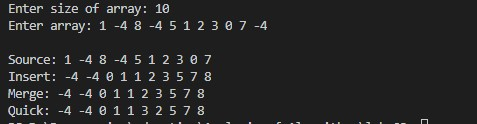
\includegraphics[scale=0.8]{example.jpg}
		\caption{Пример работы программы}
		\label{pic:example}
	\end{figure}
	
	\section{Сравнение времени работы алгоритмов}
	\subsection{Лучшее время}
	Для сравнения лучшего времени работы алгоритмов сортировки массивов были использованы отсортированные массивы длиной от 100 до 1000 с шагом 50. Эксперимент для более точного результата повторялся 1000 раз. Итоговый результат рассчитывался как средний из полученных результатов. Результаты измерений показаны в таблице \ref{table-time} и на рисунке \ref{graph-time}.\\
	\begin{table}[ht!]
		\caption{Лучшее время работы алгоритмов сортировки массивов в тактах процессора}
		\label{table-time}
		\begin{center}
			\pgfplotstabletypeset[
			col sep=semicolon,
			string type,
			columns/Size/.style={column name=Размер массива, column type={|c}},
			columns/Insert/.style={column name=Сортировка вставками, column type={|c}},
			columns/Merge/.style={column name=Сортировка слиянием, column type={|c}},
			columns/Quick/.style={column name=Быстрая сортировка, column type={|c|}},
			every head row/.style={before row=\hline,after row=\hline},
			every last row/.style={after row=\hline},
			]{AscTime.csv}
		\end{center}
	\end{table}
	
	\begin{figure}[ht!]
		\begin{tikzpicture}
		\begin{axis}
			[%title = График времени работы алгоритмов сортировки массивов,
			table/col sep = semicolon,
			xlabel={Размер массивов},
			ylabel={Время в тиках},
			ymin = 0,
			legend pos=outer north east,
			ymajorgrids=true,
			grid style=dashed]
			\addplot[color=red, mark=*] table[x={Size}, y={Insert}] {AscTime.csv};
			\addplot[color=blue, mark=*] table[x={Size}, y={Merge}] {AscTime.csv};
			\addplot[color=green, mark=*] table[x={Size}, y={Quick}] {AscTime.csv};
			\legend{Сортировка вставками, Сортировка слиянием, Быстрая сортировка}
		\end{axis}
		\end{tikzpicture}
		\caption{График лучшего времени работы алгоритмов сортировки массивов}
		\label{graph-time}
	\end{figure}

	Можно заметить, что при уже отсортированном массиве на входе по времени выигрывает самый простой в реализации алгоритм - сортировка вставками, он быстрее быстрой сортировки в 10 раз, а сортировки слиянием - в 50 раз. Также можно заметить, что алгоритм сортировки слиянием значительно проигрывает по времени двум другим алгоритмам из-за большого числа сравнений, которое выполняется в данном алгоритме независимо от входных данных.

	\newpage
	
	\subsection{Среднее время}
	Для сравнения среднего времени работы алгоритмов сортировки массивов были использованы случайно сгенерированные массивы длиной от 100 до 1000 с шагом 50. Эксперимент для более точного результата повторялся 1000 раз. Итоговый результат рассчитывался как средний из полученных результатов. Результаты измерений показаны в таблице \ref{table2-time} и на рисунке \ref{graph2-time}.\\
	\begin{table}[ht!]
		\caption{Среднее время работы алгоритмов сортировки массивов в тактах процессора}
		\label{table2-time}
		\begin{center}
			\pgfplotstabletypeset[
			col sep=semicolon,
			string type,
			columns/Size/.style={column name=Размер массива, column type={|c}},
			columns/Insert/.style={column name=Сортировка вставками, column type={|c}},
			columns/Merge/.style={column name=Сортировка слиянием, column type={|c}},
			columns/Quick/.style={column name=Быстрая сортировка, column type={|c|}},
			every head row/.style={before row=\hline,after row=\hline},
			every last row/.style={after row=\hline},
			]{RandTime.csv}
		\end{center}
	\end{table}
	
	\begin{figure}[ht!]
		\begin{tikzpicture}
		\begin{axis}
		[%title = График времени работы алгоритмов сортировки массивов,
		table/col sep = semicolon,
		xlabel={Размер массивов},
		ylabel={Время в тиках},
		ymin = 0,
		legend pos=outer north east,
		ymajorgrids=true,
		grid style=dashed]
		\addplot[color=red, mark=*] table[x={Size}, y={Insert}] {RandTime.csv};
		\addplot[color=blue, mark=*] table[x={Size}, y={Merge}] {RandTime.csv};
		\addplot[color=green, mark=*] table[x={Size}, y={Quick}] {RandTime.csv};
		\legend{Сортировка вставками, Сортировка слиянием, Быстрая сортировка}
		\end{axis}
		\end{tikzpicture}
		\caption{График среднего времени работы алгоритмов сортировки массивов}
		\label{graph2-time}
	\end{figure}

	По среднему времени рекурсивные алгоритмы выигрывают простую сортировку вставками, что следует из трудоёмкости алгоритмов. Разница во времени растёт с увеличением размера массива: так при размере массива 500 сортировкой вставками медленее сортировки слиянием в 2,2 раза, а при размере 100 - в 4 раза. При этом можно заметить, что алгоритм сортировки вставками работает примерно за то же время, что и алгоритм сортировки слиянием, при размерах, меньших 200. Сортировками слиянием в среднем работает в 2 раза медленнее быстрой сортировки.

	\newpage
	
	\subsection{Худшее время}
	Для сравнения среднего времени работы алгоритмов сортировки массивов были использованы отсортированные в обратном порядке массивы длиной от 100 до 1000 с шагом 50. Эксперимент для более точного результата повторялся 1000 раз. Итоговый результат рассчитывался как средний из полученных результатов. Результаты измерений показаны в таблице \ref{table3-time} и на рисунке \ref{graph3-time}.\\
	\begin{table}[ht!]
		\caption{Худшее время работы алгоритмов сортировки массивов в тактах процессора}
		\label{table3-time}
		\begin{center}
			\pgfplotstabletypeset[
			col sep=semicolon,
			string type,
			columns/Size/.style={column name=Размер массива, column type={|c}},
			columns/Insert/.style={column name=Сортировка вставками, column type={|c}},
			columns/Merge/.style={column name=Сортировка слиянием, column type={|c}},
			columns/Quick/.style={column name=Быстрая сортировка, column type={|c|}},
			every head row/.style={before row=\hline,after row=\hline},
			every last row/.style={after row=\hline},
			]{DescTime.csv}
		\end{center}
	\end{table}
	
	\begin{figure}[ht!]
		\begin{tikzpicture}
		\begin{axis}
		[%title = График времени работы алгоритмов сортировки массивов,
		table/col sep = semicolon,
		xlabel={Размер массивов},
		ylabel={Время в тиках},
		ymin = 0,
		legend pos=outer north east,
		ymajorgrids=true,
		grid style=dashed]
		\addplot[color=red, mark=*] table[x={Size}, y={Insert}] {DescTime.csv};
		\addplot[color=blue, mark=*] table[x={Size}, y={Merge}] {DescTime.csv};
		\addplot[color=green, mark=*] table[x={Size}, y={Quick}] {DescTime.csv};
		\legend{Сортировка вставками, Сортировка слиянием, Быстрая сортировка}
		\end{axis}
		\end{tikzpicture}
		\caption{График худшего времени работы алгоритмов сортировки массивов}
		\label{graph3-time}
	\end{figure}

	В худшем случае лишь увеличивается разница во времени выполнения: сортировка слиянием работает медленее быстрой сортировки в 5 раз, при размере массива 500 сортировкой вставками медленее сортировки слиянием в 6,2 раза, а при размере 100 - в 12 раз.

	\chapter*{Заключение}
	\addcontentsline{toc}{chapter}{Заключение}
	
	В ходе лабораторной работы были изучены и реализованы три алгоритма сортировки: вставками, слиянием и быстрая сортировка. Был проведён сравнительный анализ алгоритмов, который показал, что при различных исходных данных применительны каждый из данных алгоритмов сортировки. Также экспериментально были подтверждены временные различия в работе алгоритмов.
	
	\newpage
	
	\begin{thebibliography}{}
	\bibitem{Merge} Левитин А. В. Глава 4. Метод декомпозиции: Сортировка слиянием // Алгоритмы. Введение в разработку и анализ — М.: Вильямс, 2006
	\bibitem{Quick} Левитин А. В. Глава 4. Метод декомпозиции: Быстрая сортировка // Алгоритмы. Введение в разработку и анализ — М.: Вильямс, 2006
	\bibitem{AlgAnalysis} Кормен, Т. Алгоритмы: построение и анализ / Т. Кормен, Ч. Лейзерсон, Р.М. Ривест: – МЦНТО, 1999.
	\bibitem{CPP} https://cppreference.com/ [Электронный ресурс]
	\end{thebibliography}
	\addcontentsline{toc}{chapter}{Литература}

\end{document}
